Nach einer erfolgreichen Einrichtung kann der Nutzer sich in Zukunft mithilfe des neuen Konzepts einfacher authentisieren bei Eingabe des zweiten Faktors (dem TOTP). Das Konzept sieht dabei den in Abb. \ref{fig: konzept login} dargestellten Ablauf vor.

\begin{figure}
    \centering
    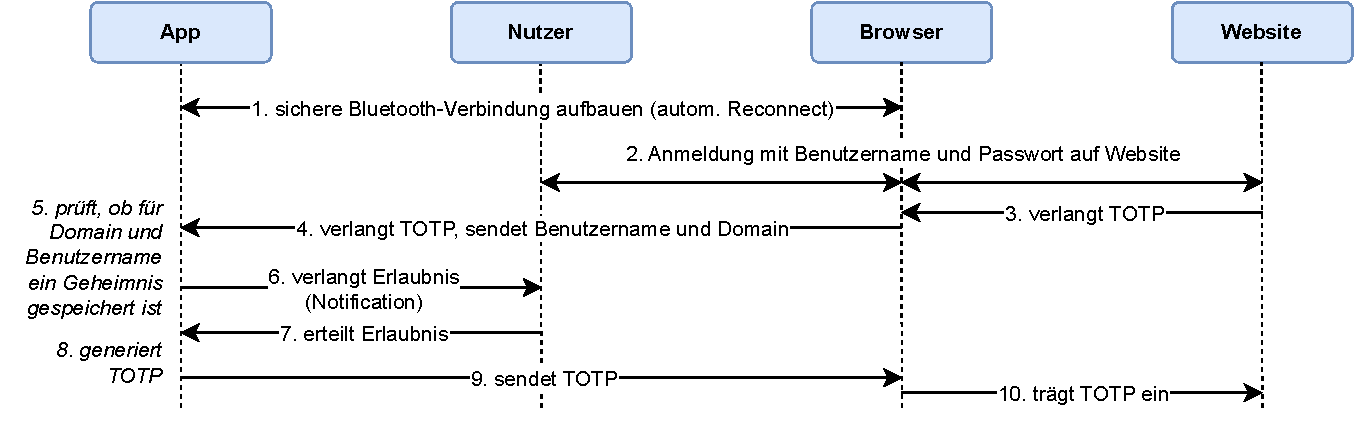
\includegraphics[width=1\linewidth]{figures/konzept_login.pdf}
    \caption[Authentisierungsvorgang des Konzepts zu einem neuen TOTP-Verfahren]{Authentisierungsvorgang des Konzepts zu einem neuen TOTP-Verfahren}
    \label{fig: konzept login}
\end{figure}

\paragraph*{Aufbau einer sicheren Bluetooth-Verbindung (1.)}
\mbox{} \vspace{0.1cm} \\
Wie bereits bei der Einrichtung beschrieben, bauen App und Browser eine sichere 
Bluetooth-Verbindung auf. Es ist von Vorteil, wenn Bluetooth sowohl auf dem 
Smartphone als auch auf dem Computer aktiviert ist, damit App und Browser sich 
ohne eine weitere Nutzerinteraktion automatisch neu verbinden. Des Weiteren senkt 
es die Nutzerinterkationen, wenn die App immer im Hintergrund läuft, damit der 
Nutzer die App nicht öffnen muss, nur um sie mit dem Browser zu verbinden.

\paragraph*{Anmeldung mit Benutzername und Passwort (2.)}
\mbox{} \vspace{0.1cm} \\
Wie gewohnt meldet sich der Nutzer mit Benutzername und Passwort bei der Website 
an und erfüllt somit den ersten Faktor der 2FA.

\paragraph*{Verlangen des TOTPs (3. - 5.)}
\mbox{} \vspace{0.1cm} \\
Wie bereits bei der Einrichtung beschrieben, kann der Browser das Eingabeelement 
des Benutzernamens durch den HTML-Quellcode erkennen. Mit dem HTML-Attribut  
\lstinline{autocomplete="one-time-code"} kann der Browser auch das Eingabeelement des 
Einmalpassworts erkennen. Allerdings ist bei Webdiensten der Gebrauch des 
Attributwertes \lstinline{one-time-code} nicht so sehr vertreten wie \lstinline{username}. D.h. Webdienste müssen konsequent das Eingabeelement des TOTPs 
markieren, damit das Konzept funktioniert.
Hat der Browser das TOTP-Eingabeelement erkannt, verlangt der das TOTP von der 
App. Zusätzlich übergibt er Benutzername und Domain, damit die App das zugehörige 
Geheimnis in ihrem Speicher identifizieren kann. Im Fall, dass der Nutzer sich auf einer Phishing-Website befindet, würde die App kein Geheimnis in ihrem Speicher finden, da sie nur die Domain der echten Website kennt und nicht die Domain der Phishing-Website. Demnach kann die App auch kein TOTP generieren und warnt den Nutzer.

\paragraph*{Freigabe des TOTPs durch den Nutzer (6. \& 7.)}
\mbox{} \vspace{0.1cm} \\
Besitzt die App ein Geheimnis für die empfangene Domain und den zugehörigen Benutzernamen, dann fragt sie den Nutzer um Erlaubnis für die Übertragung des 
TOTPs an den Browser. Über eine Notification kann die Anfrage an den Nutzer 
gestellt werden. Je nach Betriebssystem kann der Nutzer direkt mit der 
Notification interagieren und so die Anfrage bestätigen und ablehnen, ohne die 
App öffnen zu müssen \autocite{appleNotify,androidNotify}. 
Diese Schritte zur Freigabe des TOTPs sind nur für den Fall notwendig, dass der 
Browser durch Malware kompromittiert wurde oder dass es einem Angreifer in der 
Nähe durch eine Sicherheitslücke gelingt, sich als vertrauter Browser auszugeben. 
In einem solchen Fall ist die Bedrohung für den Nutzer nicht zwingend 
offensichtlich, aber anhand des Zeitpunktes des Empfangens der Notification, weiß 
der Nutzer, ob diese Anfrage von ihm stammt oder nicht. Ausnahme ist hier der 
Fall, dass der Angreifer gezielt zur selben Zeit wie der Browser des Nutzers das 
TOTP von der App verlangt.

\paragraph*{Übertragung des TOTPs an die Website (8. - 10.)}
\mbox{} \vspace{0.1cm} \\
Die App generiert nun das TOTP und sendet es an den Browser. Dieser trägt es dann 
automatisch in das TOTP-Eingabeelement ein. Theoretisch könnte Schritt 10 auch 
gänzlich im Hintergrund geschehen, so dass der Nutzer das Eingabefeld nie 
wahrnehmen muss.

\paragraph*{Anmerkung: Smartwatch als 5. Partei}
\mbox{} \vspace{0.1cm} \\
Verknüpft man sein Smartphone mit einer Smartwatch, kann man für gewisse Situationen annehmen, noch mehr Zeit zu sparen. Ist das Smartphone bspw. in der Tasche oder der Hostentasche, bestätigt man die Notification aus Schritt 6 mit Hilfe der Smartwatch.